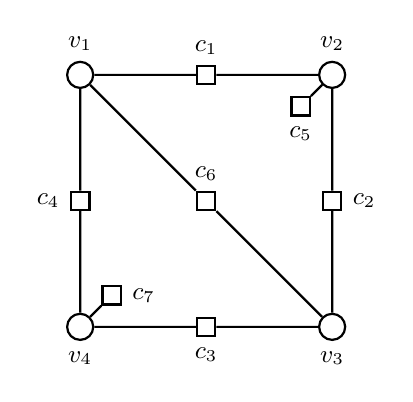
\begin{tikzpicture}[thick,scale=.8]
\node[circle,draw=black,label={above:\small{$v_1$}}] (v1) at (-2,2){};
\node[circle,draw=black,label={above:\small{$v_2$}}] (v2) at (2,2){};
\node[circle,draw=black,label={below:\small{$v_3$}}] (v3) at (2,-2){};
\node[circle,draw=black,label={below:\small{$v_4$}}] (v4) at (-2,-2){};
%\node[circle,draw=black,label={above:\small{$v_5$}}] (v5) at (0,0){};

\node[shape=rectangle,draw=black,label={above:\small{$c_1$}}] (c1) at (0,2){};
\node[shape=rectangle,draw=black,label={right:\small{$c_2$}}] (c2) at (2,0){};
\node[shape=rectangle,draw=black,label={below:\small{$c_3$}}] (c3) at (0,-2){};
\node[shape=rectangle,draw=black,label={left:\small{$c_4$}}] (c4) at (-2,0){};
\node[shape=rectangle,draw=black,label={above:\small{$c_6$}}] (c6) at (0,0){};
%\node[shape=rectangle,draw=black,label={left:\small{$c_5$}}] (c5) at (-1,1){};
%\node[shape=rectangle,draw=black,label={left:\small{$c_6$}}] (c6) at (1,-1){};
%\node[shape=rectangle,draw=black,label={left:\small{$c_7$}}] (c7) at (-.5,-.5){};
\node[shape=rectangle,draw=black,label={below:\small{$c_5$}}] (c5) at (1.5,1.5){};
\node[shape=rectangle,draw=black,label={right:\small{$c_7$}}] (c7) at (-1.5,-1.5){};

\path [-,thick] (v1) edge node[left] {} (c1); \path [-,thick] (c1) edge node[left] {} (v2);
\path [-,thick] (v1) edge node[left] {} (c4); \path [-,thick] (c4) edge node[left] {} (v4);
\path [-,thick] (v4) edge node[left] {} (c3); \path [-,thick] (c3) edge node[left] {} (v3);
\path [-,thick] (v2) edge node[left] {} (c2); \path [-,thick] (c2) edge node[left] {} (v3);
\path [-,thick] (v1) edge node[left] {} (c6); \path [-,thick] (c6) edge node[left] {} (v3);
%\path [-,thick] (v5) edge node[left] {} (c6); \path [-,thick] (c6) edge node[left] {} (v3);
%\path [-,thick] (v5) edge node[left] {} (c7);
\path [-,thick] (v2) edge node[left] {} (c5);
\path [-,thick] (v4) edge node[left] {} (c7);

\end{tikzpicture}